%%%%%%%%%%%%%%%%%%%%%%%%%%%%%%%%%%%%%%%%%
% Beamer Presentation
% LaTeX Template
% Version 2.0 (March 8, 2022)
%
% This template originates from:
% https://www.LaTeXTemplates.com
%
% Author:
% Vel (vel@latextemplates.com)
%
% License:
% CC BY-NC-SA 4.0 (https://creativecommons.org/licenses/by-nc-sa/4.0/)
%
%%%%%%%%%%%%%%%%%%%%%%%%%%%%%%%%%%%%%%%%%

%----------------------------------------------------------------------------------------
%	PACKAGES AND OTHER DOCUMENT CONFIGURATIONS
%----------------------------------------------------------------------------------------

\documentclass[
	12pt, % Set the default font size, options include: 8pt, 9pt, 10pt, 11pt, 12pt, 14pt, 17pt, 20pt
	%t, % Uncomment to vertically align all slide content to the top of the slide, rather than the default centered
	%aspectratio=169, % Uncomment to set the aspect ratio to a 16:9 ratio which matches the aspect ratio of 1080p and 4K screens and projectors
]{beamer}

\graphicspath{{Images/}{./}} % Specifies where to look for included images (trailing slash required)

\usepackage{booktabs} % Allows the use of \toprule, \midrule and \bottomrule for better rules in tables

\usepackage[dvipsnames]{xcolor}
%----------------------------------------------------------------------------------------
%	SELECT LAYOUT THEME
%----------------------------------------------------------------------------------------

% Beamer comes with a number of default layout themes which change the colors and layouts of slides. Below is a list of all themes available, uncomment each in turn to see what they look like.

%\usetheme{default}
%\usetheme{AnnArbor}
%\usetheme{Antibes}
%\usetheme{Bergen}
%\usetheme{Berkeley}
%\usetheme{Berlin}
\usetheme{Boadilla}
%%%%%%%%%\usetheme{CambridgeUS}
%\usetheme{Copenhagen}
%\usetheme{Darmstadt}
%\usetheme{Dresden}
%\usetheme{Frankfurt}
%\usetheme{Goettingen}
%\usetheme{Hannover}
%\usetheme{Ilmenau}
%\usetheme{JuanLesPins}
%\usetheme{Luebeck}
%%%%%\usetheme{Madrid}
%\usetheme{Malmoe}
%\usetheme{Marburg}
%\usetheme{Montpellier}
%\usetheme{PaloAlto}
%\usetheme{Pittsburgh}
%\usetheme{Rochester}
%\usetheme{Singapore}
%\usetheme{Szeged}
%\usetheme{Warsaw}

%----------------------------------------------------------------------------------------
%	SELECT COLOR THEME
%----------------------------------------------------------------------------------------

% Beamer comes with a number of color themes that can be applied to any layout theme to change its colors. Uncomment each of these in turn to see how they change the colors of your selected layout theme.

%\usecolortheme{albatross}
\usecolortheme{beaver}
%\usecolortheme{beetle}
%\usecolortheme{crane}
%\usecolortheme{dolphin}
%\usecolortheme{dove}
%\usecolortheme{fly}
%%%%%%%%\usecolortheme{lily}
%\usecolortheme{monarca}
%\usecolortheme{seagull}
%\usecolortheme{seahorse}
%\usecolortheme{spruce}
%\usecolortheme{whale}
%\usecolortheme{wolverine}

%----------------------------------------------------------------------------------------
%	SELECT FONT THEME & FONTS
%----------------------------------------------------------------------------------------

% Beamer comes with several font themes to easily change the fonts used in various parts of the presentation. Review the comments beside each one to decide if you would like to use it. Note that additional options can be specified for several of these font themes, consult the beamer documentation for more information.

\usefonttheme{default} % Typeset using the default sans serif font
%\usefonttheme{serif} % Typeset using the default serif font (make sure a sans font isn't being set as the default font if you use this option!)
%\usefonttheme{structurebold} % Typeset important structure text (titles, headlines, footlines, sidebar, etc) in bold
%\usefonttheme{structureitalicserif} % Typeset important structure text (titles, headlines, footlines, sidebar, etc) in italic serif
%\usefonttheme{structuresmallcapsserif} % Typeset important structure text (titles, headlines, footlines, sidebar, etc) in small caps serif

%------------------------------------------------

%\usepackage{mathptmx} % Use the Times font for serif text
\usepackage{palatino} % Use the Palatino font for serif text

%\usepackage{helvet} % Use the Helvetica font for sans serif text
\usepackage[default]{opensans} % Use the Open Sans font for sans serif text
%\usepackage[default]{FiraSans} % Use the Fira Sans font for sans serif text
%\usepackage[default]{lato} % Use the Lato font for sans serif text
\definecolor{grayhover}{rgb}{0.5, 0.5, 0.5}
%----------------------------------------------------------------------------------------
%	SELECT INNER THEME
%----------------------------------------------------------------------------------------

% Inner themes change the styling of internal slide elements, for example: bullet points, blocks, bibliography entries, title pages, theorems, etc. Uncomment each theme in turn to see what changes it makes to your presentation.

%\useinnertheme{default}
\useinnertheme{circles}
%\useinnertheme{rectangles}
%\useinnertheme{rounded}
%\useinnertheme{inmargin}

%----------------------------------------------------------------------------------------
%	SELECT OUTER THEME
%----------------------------------------------------------------------------------------

% Outer themes change the overall layout of slides, such as: header and footer lines, sidebars and slide titles. Uncomment each theme in turn to see what changes it makes to your presentation.

\useoutertheme{default}
%\useoutertheme{infolines}
%\useoutertheme{miniframes}
%\useoutertheme{smoothbars}
%\useoutertheme{sidebar}
%\useoutertheme{split}
%\useoutertheme{shadow}
%\useoutertheme{tree}
%\useoutertheme{smoothtree}

%\setbeamertemplate{footline} % Uncomment this line to remove the footer line in all slides
%\setbeamertemplate{footline}[page number] % Uncomment this line to replace the footer line in all slides with a simple slide count

%\setbeamertemplate{navigation symbols}{} % Uncomment this line to remove the navigation symbols from the bottom of all slides

%----------------------------------------------------------------------------------------
%	PRESENTATION INFORMATION
%----------------------------------------------------------------------------------------

\title[PagPassGPT]{PagPassGPT} % The short title in the optional parameter appears at the bottom of every slide, the full title in the main parameter is only on the title page

\subtitle{Pattern Guided Password Guessing
	via Generative Pretrained Transformer} % Presentation subtitle, remove this command if a subtitle isn't required

\author[Reza Adinepour]{Reza Adinepour} % Presenter name(s), the optional parameter can contain a shortened version to appear on the bottom of every slide, while the main parameter will appear on the title slide

\institute[AUT]{Amirkabir University of Technology\\ (Tehran Polytechnic) \\ \smallskip } % Your institution, the optional parameter can be used for the institution shorthand and will appear on the bottom of every slide after author names, while the required parameter is used on the title slide and can include your email address or additional information on separate lines

\date[\today]{Computer Engineering Department \\ \today} % Presentation date or conference/meeting name, the optional parameter can contain a shortened version to appear on the bottom of every slide, while the required parameter value is output to the title slide

%----------------------------------------------------------------------------------------

\begin{document}

%----------------------------------------------------------------------------------------
%	TITLE SLIDE
%----------------------------------------------------------------------------------------

\begin{frame}
	\titlepage % Output the title slide, automatically created using the text entered in the PRESENTATION INFORMATION block above
	\centering
\includegraphics[scale=0.12]{Images/Logo/logo2.png}
\end{frame}

%----------------------------------------------------------------------------------------
%	TABLE OF CONTENTS SLIDE
%----------------------------------------------------------------------------------------

% The table of contents outputs the sections and subsections that appear in your presentation, specified with the standard \section and \subsection commands. You may either display all sections and subsections on one slide with \tableofcontents, or display each section at a time on subsequent slides with \tableofcontents[pausesections]. The latter is useful if you want to step through each section and mention what you will discuss.

\begin{frame}
	\frametitle{Agenda} % Slide title, remove this command for no title
	
	\tableofcontents % Output the table of contents (all sections on one slide)
	%\tableofcontents[pausesections] % Output the table of contents (break sections up across separate slides)
\end{frame}



%----------------------------------------------------------------------------------------
%	PRESENTATION BODY SLIDES
%----------------------------------------------------------------------------------------

\section{Introduction} % Sections are added in order to organize your presentation into discrete blocks, all sections and subsections are automatically output to the table of contents as an overview of the talk but NOT output in the presentation as separate slides

%------------------------------------------------
%\subsection{Road Map}
%\begin{frame}
%	\frametitle{Road Map}
%	
%	\begin{itemize}
%		\item \textbf{Problem:} Shrinking transistor sizes lead to an increased soft error rate in computer systems, posing a significant risk of severe failures.
%		
%		
%		\item \textbf{Solution:} Introduce Error Detection by Duplicating Instruction (EDDI) at the assembly level.
%		
%		\item \textbf{Main Contribution:}
%		\begin{itemize}
%			\item FERRUM: An enhanced version of EDDI using SIMD and compiler optimizations.
%			\item 100\% fault coverage at the assembly level.
%			\item Over 50\% reduction in runtime overhead compared to existing techniques.
%		\end{itemize}
%	\end{itemize}
%	
%\end{frame}

%------------------------------------------------
\subsection{Problem \& Solutions Overview}
\begin{frame}
	\frametitle{Problem \& Solutions Overview}
	
	\begin{enumerate}
		\item \textbf{Problem:}
		Deep learning-based password guessing models face challenges in:
		\begin{itemize}
			\item Generating high-quality passwords.
			\item Reducing the rate of duplicate passwords.
		\end{itemize}
		
		\item \textbf{Impact:}
		Reduced efficiency in password guessing models due to:
		\begin{itemize}
			\item Lower hit rates.
			\item High redundancy in generated passwords, limiting practical effectiveness.
		\end{itemize}
	\end{enumerate}
\end{frame}





\begin{frame}
	\frametitle{Solutions}
	

	\begin{enumerate}
		\item PagPassGPT:
		\begin{itemize}
			\item Built on a Generative Pretrained Transformer (GPT).
			\item Incorporates pattern structure information as background knowledge to improve guessing accuracy.
		\end{itemize}
		
		\item D\&C-GEN (Divide-and-Conquer Generation):
		\begin{itemize}
			\item Divides password guessing tasks into non-overlapping subtasks.
			\item Subtasks inherit parent task knowledge for efficient prediction.
			\item Effectively reduces duplicate passwords.
		\end{itemize}
		
		\item Results:
		\begin{itemize}
			\item 12\% higher hit rate compared to state-of-the-art models.
			\item 25\% fewer duplicate passwords.
		\end{itemize}
	\end{enumerate}
\end{frame}



\section{Main Contribution}
\begin{frame}
	\frametitle{Main Contribution}
	
	\begin{enumerate}
		\item \textbf{PagPassGPT:} 
		\begin{itemize}
			\item Combines password patterns with deep learning.
			\item Improves guessing accuracy.
		\end{itemize}
		
		\item \textbf{D\&C-GEN:}
		\begin{itemize}
			\item Uses divide-and-conquer for task splitting.
			\item Reduces duplicate passwords.
		\end{itemize}
		
		\item \textbf{Performance:}
		\begin{itemize}
			\item Validated on public datasets.
			\item Outperforms state-of-the-art models in hit rate and duplicates.
		\end{itemize}
	\end{enumerate}
\end{frame}



\section{Related Works}
\begin{frame}
	\frametitle{Related works}
	
	\begin{enumerate}
		\item \textbf{Password Guessing Types}
		\begin{itemize}
			\item Trawling Attack:\\
			\textcolor{red}{Problem:} Misses rate patterns; requires accurate modeling.
			
			\item Targeted Attack:\\
			\textcolor{red}{Problem:} Depends on personally identifiable information (PII); less effective with unpredictable users.
		\end{itemize}
		
		
		\item \textbf{Password Guessing Models}
		\begin{itemize}
			\item Rule-based Models:\\
			\textcolor{red}{Problem:} Background knowledge dependency; limited rules.
			
			\item Probability-based Models:\\
			\textcolor{red}{Problem:} Fixed vocabulary; poor segmentation accuracy.
		\end{itemize}
		
		
		\item \textbf{Deep Learning-based Models:}\\
		\textcolor{red}{Problem:} Accuracy loss; high computation.
		
	\end{enumerate}
\end{frame}



%------------------------------------------------

\section{PagPass Methods}
\begin{frame}
	\frametitle{PagPass Methods}
	
	\begin{figure}
		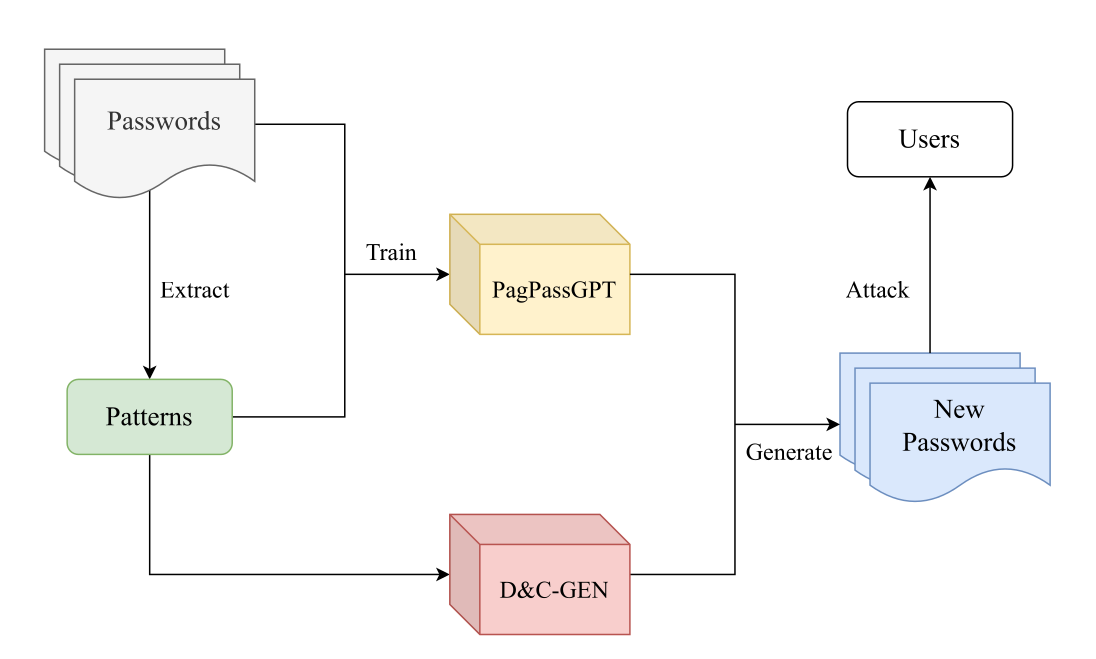
\includegraphics[width=0.9\linewidth]{img1.png}
		\caption{High-level idea of EDDI}
		\label{High-level idea of EDDI}
	\end{figure}
\end{frame}




\begin{frame}
	\frametitle{Training Process}
	\begin{enumerate}
		\item \textbf{Input:} Passwords from a training dataset.
		\item \textbf{Training:}
		\begin{itemize}
			\item Extract password patterns (e.g., "L4N3S1") using PCFG rules.
			\item Combine patterns and passwords into a structured sequence:
			\texttt{<BOS> || Pattern || <SEP> || Password || <EOS>}
			\item Tokenize sequences and embed using GPT-2 architecture.
			\item Optimize with cross-entropy loss for improved prediction accuracy.
		\end{itemize}
	\end{enumerate}
\end{frame}




\begin{frame}
	\frametitle{Training Process (Cont.)}
	
	% TODO: \usepackage{graphicx} required
	\begin{figure}
		\centering
		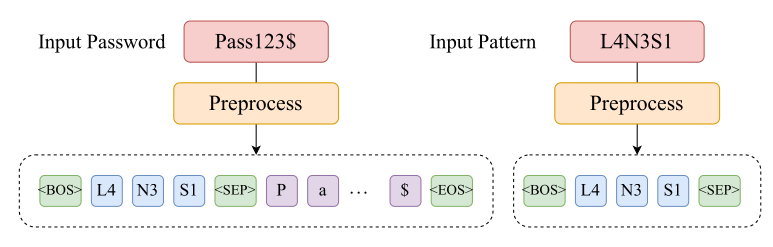
\includegraphics[width=0.9\linewidth]{Images/img4}
		\caption{The preprocessing operation of tokenizer of PagPassGPT}
		\label{fig:The preprocessing operation of tokenizer of PagPassGPT}
	\end{figure}
\end{frame}




\begin{frame}
	\frametitle{Training Process (Cont.)}
	
	% TODO: \usepackage{graphicx} required
	\begin{figure}
		\centering
		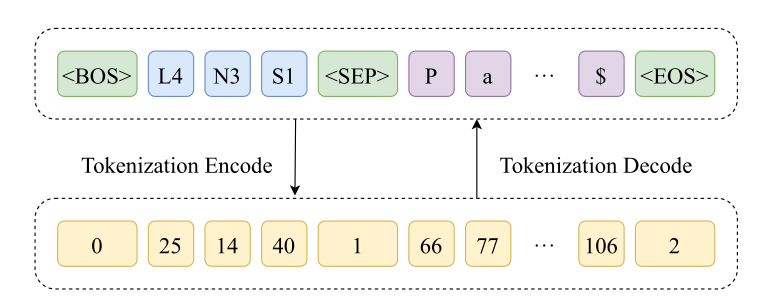
\includegraphics[width=0.9\linewidth]{Images/img5}
		\caption{The tokenization process of the tokenizer of PagPassGPT}
		\label{fig:The tokenization process of the tokenizer of PagPassGPT}
	\end{figure}
\end{frame}



\begin{frame}
	\frametitle{Training Process (Cont.)}
	
	% TODO: \usepackage{graphicx} required
	\begin{figure}
		\centering
		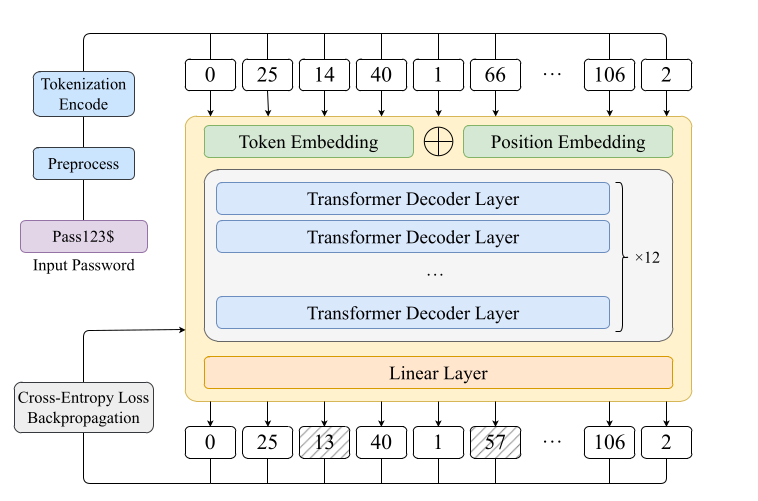
\includegraphics[width=0.8\linewidth]{Images/img2}
		\caption{Training process architecture}
		\label{fig:Training process architecture}
	\end{figure}
\end{frame}













%
%\begin{frame}
%	\frametitle{Training Process (Cont.)}
%	\begin{enumerate}
%	\item \textbf{Generation:}
%	\begin{itemize}
%		\item Predict tokens sequentially using an auto-regressive mechanism based on:
%		\begin{itemize}
%			\item Historical tokens.
%			\item Password patterns.
%		\end{itemize}
%		\item Achieves 27.5\% higher hit rate compared to PassGPT.
%	\end{itemize}
%\end{enumerate}
%\end{frame}





\begin{frame}
	\frametitle{D\&C-GEN}
	
	\begin{enumerate}
		\item \textbf{Objective:} Reduce duplicate passwords using divide-and-conquer.
		
		\item \textbf{Workflow:}
		\begin{itemize}
			\item Split tasks into non-overlapping subtasks by patterns and prefixes.
			\item Apply a threshold $T$ to stop division and execute generation.
			\item Generate passwords efficiently under task constraints.
		\end{itemize}
		
		\item \textbf{Performance:}
		\begin{itemize}
			\item Reduces duplicate rate to 9.28\% for $10^9$ guesses.
			\item Supports parallel execution and optimized GPU utility.
		\end{itemize}
	\end{enumerate}
\end{frame}


%\subsection{Example Code}
\begin{frame}
	\frametitle{D\&C-GEN (Cont.)}
	
	
	% TODO: \usepackage{graphicx} required
	\begin{figure}
		\centering
		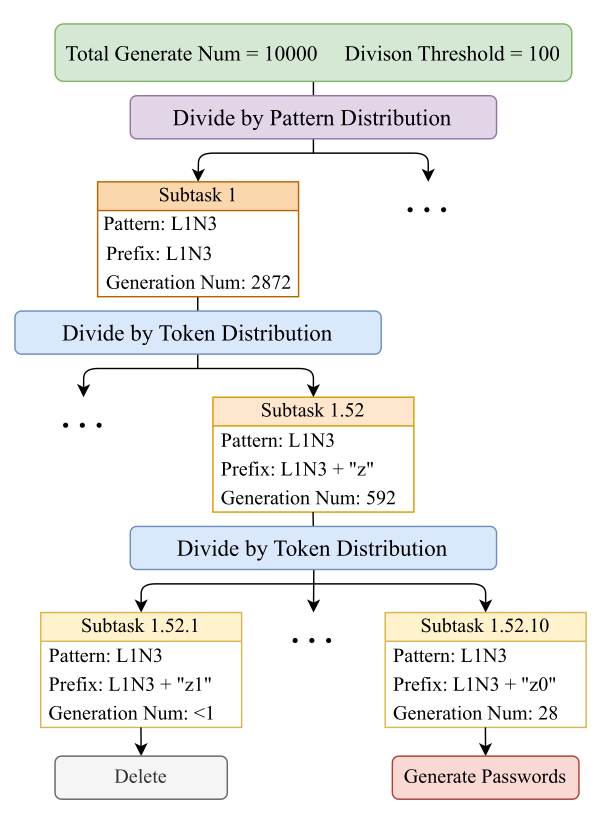
\includegraphics[width=0.5\linewidth]{Images/img6}
		\caption{The workflow of D\&C-GEN}
		\label{fig:The workflow of D&C-GEN}
	\end{figure}
	
\end{frame}


%------------------------------------------------



%------------------------------------------------









\section{Evaluation}
\begin{frame}
	\frametitle{Evaluation}
	
	\begin{enumerate}
		\item \textbf{Datasets}
		\begin{itemize}
			\item Ethical Considerations:
			\begin{itemize}
				\item Public data, minimal usage, and strictly for research purposes.
			\end{itemize}
			
			\item Applied Datasets:
			\begin{itemize}
				\item RockYou, LinkedIn, phpBB, MySpace, Yahoo!
				\item Total entries: 75,349,874.
			\end{itemize}
			
			\item Data Cleaning:
			\begin{itemize}
				\item Password length: 4–12 characters.
				\item Removed duplicates and non-ASCII characters.
			\end{itemize}
			
			\item Data Utilization:
			\begin{itemize}
				\item RockYou \& LinkedIn: Split into training (70\%), validation (10\%), and testing (20\%).
				\item Cross-site evaluation: Used all remaining datasets.
			\end{itemize}
		\end{itemize}
	\end{enumerate}
\end{frame}




\begin{frame}
	\frametitle{Evaluation (Cont.)}
	
	\begin{enumerate}
		\item \textbf{Models}
		\begin{itemize}
			\item PagPassGPT:
			\begin{itemize}
				\item Trained with batch size 512 for 30 epochs using AdamW optimizer.
				\item Max tokens: 32, Embedding size: 256.
				\item Hidden layers: 12, Attention heads: 8.
				\item Training duration: 25+ hours on 4 RTX 3080 GPUs.
			\end{itemize}
		\end{itemize}
		
		\item \textbf{Drawling Attack Test}
		\begin{itemize}
			\item Setup:
			\begin{itemize}
				\item Compared PagPassGPT and PagPassGPT-D\&C (with threshold $T=4000$) against models like PassGAN, VAEPass, PassFlow, and PassGPT.
			\end{itemize}
			
		\end{itemize}
	\end{enumerate}
\end{frame}






\begin{frame}
	\frametitle{Evaluation (Cont.)}
	
	\begin{enumerate}
		\item \textbf{Metrics}
		\begin{itemize}
			\item Hit Rate:
			\begin{itemize}
				\item Ratio of correctly guessed passwords to total test set passwords.
				\item PagPassGPT-D\&C achieved a 53.63\% hit rate for $10^9$ guesses, 12\% higher than PassGPT.
			\end{itemize}
			
			\item Repeat Rate:
			\begin{itemize}
				\item Reflects duplicate passwords among generated ones.
				\item PagPassGPT-D\&C achieved a 9.28\% repeat rate, significantly lower than PassGPT’s 34.5\%.
			\end{itemize}
%			
%			
%			\item Length and Pattern Distribution:
%			\begin{itemize}
%				\item Length Distance: 4.78\% (half of PassGPT's 9.16\%).
%				\item Pattern Distance: 2.79\% (lower than PassGPT's 4.16\%).
%			\end{itemize}
		\end{itemize}
	\end{enumerate}
\end{frame}









\section{Results}
\subsection{Hit Rate}
\begin{frame}
	\frametitle{Hit Rate}
	

	\begin{table}[h]
		\centering
		\caption{Hit rates of different models in trawling attack test.}
		\begin{tabular}{c c c c c}
			\hline
			\textbf{Guess Num} & \textbf{$10^6$} & \textbf{$10^7$} & \textbf{$10^8$} & \textbf{$10^9$} \\ \hline \hline
			PassGAN & 0.80\% & 3.11\% & 8.24\% & 16.32\% \\ 
			VAEPass & 0.49\% & 2.24\% & 6.24\% & 12.23\% \\ 
			PassFlow & 0.26\% & 1.62\% & 7.03\% & 14.10\% \\ 
			PassGPT & 0.73\% & 5.60\% & 21.43\% & 41.93\% \\ 
			PagPassGPT & 1.00\% & 7.68\% & 27.23\% & 48.75\% \\ 
			PagPassGPT-D\&C & \textbf{1.05\%} & \textbf{8.48\%} & \textbf{31.38\%} & \textbf{53.63\%} \\ \hline
		\end{tabular}
		\label{table:hit_rates}
	\end{table}
\end{frame}




\subsection{Repeat Rate}
\begin{frame}
	\frametitle{Repeat Rate}
	
	
	% TODO: \usepackage{graphicx} required
	\begin{figure}
		\centering
		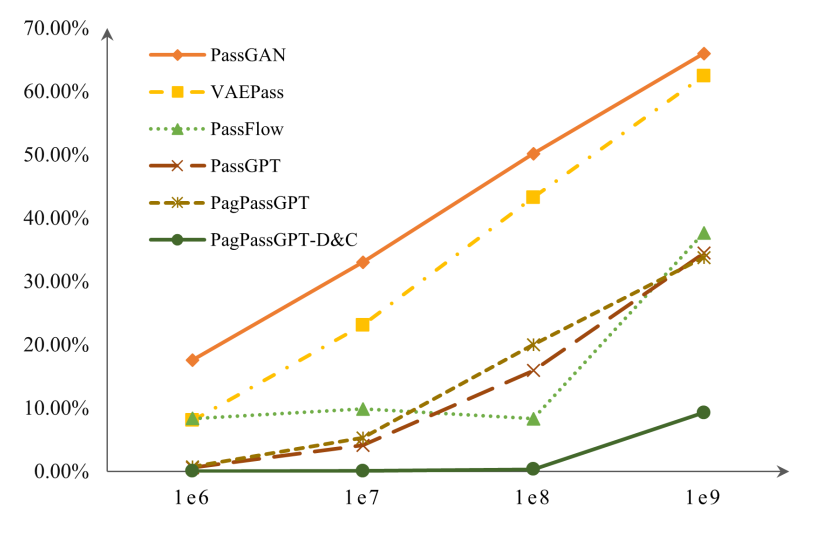
\includegraphics[width=0.8\linewidth]{Images/img7}
		\caption{Repeat rates of passwords generated by different models}
		\label{fig:Repeat rates of passwords generated by different models}
	\end{figure}
\end{frame}





%\subsection{Length distances}
%\begin{frame}
%	\frametitle{Length distances}
%	
%	
%	\begin{table}[h]
%		\centering
%		\caption{Length distances and pattern distances between passwords generated by different models and the test set.}
%		\begin{tabular}{c c c}
%			\hline
%			\textbf{Model} & \textbf{Length Distance} & \textbf{Pattern Distance} \\ \hline \hline
%			PassGAN & 9.20\% & 6.00\% \\ 
%			VAEPass & 5.84\% & 5.75\% \\ 
%			PassFlow & 50.61\% & 13.62\% \\ 
%			PassGPT & 8.49\% & 4.16\% \\ 
%			PagPassGPT & \textbf{4.78\%} & \textbf{2.79\%} \\ \hline
%		\end{tabular}
%		\label{table:length_pattern_distance}
%	\end{table}
%	
%	
%\end{frame}



\begin{frame} % Use [allowframebreaks] to allow automatic splitting across slides if the content is too long
	\frametitle{References}
	
	\begin{thebibliography}{99} % Beamer does not support BibTeX so references must be inserted manually as below, you may need to use multiple columns and/or reduce the font size further if you have many references
		\footnotesize % Reduce the font size in the bibliography
		
		\bibitem[Su et al., 2024]{p2}
		Xingyu Su, Xiaojie Zhu, Yang Li, Yong Li, Chi Chen, Paulo Esteves-Verı́ssimo (2024)
		\newblock PagPassGPT: Pattern Guided Password Guessing via Generative Pretrained Transformer
		\newblock \emph{arXiv:2404.04886v2 [cs.CR]}, School of Cyber Security, University of Chinese Academy of Sciences, Beijing, China; Institute of Information Engineering, Chinese Academy of Sciences, Beijing, China; King Abdullah University of Science and Technology, Thuwal, Kingdom of Saudi Arabia.
		\newblock Emails: \{suxingyu, liyang8119, liyong, chenchi\}@iie.ac.cn, \{xiaojie.zhu, paulo.verissimo\}@kaust.edu.sa.
		
		
		
		
	\end{thebibliography}
\end{frame}

%----------------------------------------------------------------------------------------
%	ACKNOWLEDGMENTS SLIDE
%----------------------------------------------------------------------------------------

%\begin{frame}
%	\frametitle{Acknowledgements}
%	
%	\begin{columns}[t] % The "c" option specifies centered vertical alignment while the "t" option is used for top vertical alignment
%		\begin{column}{0.45\textwidth} % Left column width
%			\textbf{Smith Lab}
%			\begin{itemize}
%				\item Alice Smith
%				\item Devon Brown
%			\end{itemize}
%			\textbf{Cook Lab}
%			\begin{itemize}
%				\item Margaret
%				\item Jennifer
%				\item Yuan
%			\end{itemize}
%		\end{column}		
%		\begin{column}{0.5\textwidth} % Right column width
%			\textbf{Funding}
%			\begin{itemize}
%				\item British Royal Navy
%				\item Norwegian Government
%			\end{itemize}
%		\end{column}
%	\end{columns}
%\end{frame}

%----------------------------------------------------------------------------------------
%	CLOSING SLIDE
%----------------------------------------------------------------------------------------

\begin{frame}[plain] % The optional argument 'plain' hides the headline and footline
	\begin{center}
		{\Huge The End}
		
		\bigskip\bigskip % Vertical whitespace
		
		{\LARGE Questions? Comments?}\vfil
		\texttt{\href{mailto:adinepour@aut.ac.ir}{\textcolor{red}{adinepour@aut.ac.ir}}}
	\end{center}
\end{frame}

%----------------------------------------------------------------------------------------

\end{document} 